% !TeX program = pdflatex
% Counting with the Derivative Tower -- the Budan-Fourier theorem in Lean 4.
% Part of the reverse-formalization line (Mathlib gaps -> formalize): the natural
% companion of Sturm's theorem, on the derivative tower instead of the remainder chain.
% Build: pdflatex budan-fourier-lean.tex (twice, for refs)
% Verified against the Lean source 2026-06-16 (lake env lean BudanFourier.lean, exit 0;
% #print axioms BudanFourier.budan_fourier -> propext, Classical.choice, Quot.sound only).
% Toolchain v4.30.0-rc2, Mathlib pin 701fb6e9. Worked examples re-checked in exact arithmetic.

\documentclass[11pt]{article}
\usepackage[T1]{fontenc}
\usepackage{lmodern}
\usepackage{amsmath,amssymb,amsthm,booktabs,graphicx,hyperref}
\usepackage{xurl}
\usepackage[table]{xcolor}
\definecolor{ggteal}{HTML}{1B6F8C}
\definecolor{ggband}{HTML}{DCE7EB}
\definecolor{ggamber}{HTML}{E08A1E}
\definecolor{ggplum}{HTML}{7B4B94}
\usepackage[margin=1in]{geometry}
\usepackage{microtype}
\usepackage{float}
\usepackage[most]{tcolorbox}
\usepackage{tikz}
\usetikzlibrary{arrows.meta,positioning}
\graphicspath{{figures/}}
\setlength{\emergencystretch}{2em}
\newtheorem{theorem}{Theorem}
\newtheorem{lemma}{Lemma}
\newtheorem{proposition}{Proposition}
\newtheorem{remark}{Remark}
\newcommand{\lean}[1]{\texttt{#1}}
\newcommand{\R}{\mathbb{R}}
\newcommand{\V}{\mathrm{V}}
\hypersetup{colorlinks=true,linkcolor=ggteal,citecolor=ggteal,urlcolor=ggteal}
\newtcbox{\keybox}{on line,boxrule=0.9pt,colframe=ggteal,colback=ggband!40,
  arc=3pt,left=8pt,right=8pt,top=5pt,bottom=5pt}
\newcommand{\keyeq}[1]{\begin{center}\keybox{$\displaystyle #1$}\end{center}}
\newtcolorbox{recipebox}[1]{colframe=ggamber,colback=ggamber!8,arc=3pt,boxrule=0.8pt,
  title=\textbf{#1},coltitle=white,colbacktitle=ggamber}

\title{\bf Counting with the Derivative Tower\\[4pt]
  \large\normalfont The Budan--Fourier theorem, machine-checked in Lean~4}
\author{Carles Mar\'in\thanks{Formalized with the assistance of an AI system (Claude,
Anthropic); the mathematics is classical, and every claim, scope statement, and limitation is
the author's responsibility. The boundary of the contribution is set out plainly in
Section~\ref{sec:boundary}, and the Lean kernel---not the assistant---is what certifies the
proofs.}\\[3pt]
  \normalsize Independent researcher\\
  \normalsize \texttt{karlesmarin@gmail.com}}
\date{June 2026}

\begin{document}
\maketitle

\begin{abstract}
I report a complete, \lean{sorry}-free formalization in Lean~4, over Mathlib, of the
\emph{Budan--Fourier theorem}: for a nonzero real polynomial $p$ and an interval $(a,b]$ whose
endpoints are not roots, the number of real roots of $p$ in $(a,b]$, \emph{counted with
multiplicity}, is at most the drop $\V(a)-\V(b)$ in the sign variations of the derivative tower
$p,\,p',\,p'',\dots,p^{(\deg p)}$, and differs from it by an even number:
\[
  \#\mathrm{roots}(a,b]\ \le\ \V(a)-\V(b),\qquad \V(a)-\V(b)-\#\mathrm{roots}(a,b]\ \text{is even.}
\]
No root is ever located; signs along a tower of derivatives are read and subtracted. The
mathematics is classical and has been formalized once before, in Isabelle/HOL by Wenda
Li~\cite{liBF}; to the best of my knowledge---based on searches of Loogle and Mathlib in
June~2026 (Section~\ref{sec:boundary})---this is the first proof of the Budan--Fourier theorem in
Lean. Mathlib carries Descartes' rule of signs (\lean{Polynomial.signVariations}, the coefficient
count) but neither the derivative tower nor the interval theorem; this work fills that gap and is
the exact companion of a recent Lean formalization of Sturm's theorem~\cite{sturmlean}, sharing its
sign-variation toolkit. The contribution is the formalization and the reusable machinery the
proof required: two one-step \emph{monotonicity bricks} that fix the sign of a derivative just off a
root, an abstract pair of list operations (\lean{Rseq}/\lean{Lseq}) that decouples the
sign-bookkeeping from the polynomials, and the identification of the leading-zero run of the tower
with the root multiplicity. The headline theorem \lean{budan\_fourier} depends only on the three
standard axioms \lean{propext}, \lean{Classical.choice}, \lean{Quot.sound}.
\end{abstract}

\medskip
\noindent\emph{What you will find here.} This is a short guided tour, not a reference manual, and it
is built like a string of beads: each section ends by handing the reader the question the next one
answers. The first asks how a difference of two integers can bound---and nearly count---the roots
(Section~\ref{sec:q1}); the second, why the count moves only at critical points, and there by the
\emph{multiplicity}, up to an even surplus (Section~\ref{sec:q2}); the third, where the proof
genuinely resists being made formal, now that the tower is no longer a coprime chain
(Section~\ref{sec:q3}); the fourth, what becomes free once the theorem is in the library---including
why Descartes' rule overcounts by an even number (Section~\ref{sec:q4}). The load-bearing lemmas are
gathered in one table (Section~\ref{sec:blocks}); the honest limits are stated without varnish in
Section~\ref{sec:boundary}; and the closing section asks, by way of reflection, the questions I
would rather carry into the next paper than pretend to have settled. If you read only two things,
read Theorem~\ref{thm:bf} and Figure~\ref{fig:tower}; the rest is the argument that connects them.

\begin{figure}[htbp]
\centering
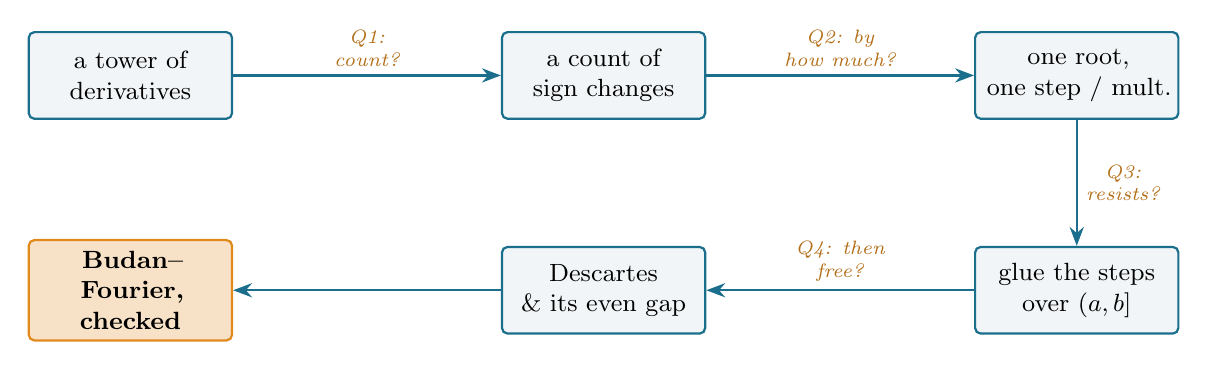
\begin{tikzpicture}[
  obj/.style={draw=ggteal,thick,rounded corners=2pt,fill=ggband!40,align=center,
    font=\small,inner sep=4pt,minimum height=11mm,text width=23mm},
  q/.style={font=\scriptsize\itshape,text=ggamber!80!black,align=center,fill=white,inner sep=1pt},
  arr/.style={-{Stealth[length=2.4mm]},thick,ggteal}]
  \node[obj] (seq) {a tower of\\derivatives};
  \node[obj,right=34mm of seq] (count) {a count of\\sign changes};
  \node[obj,right=34mm of count] (quantum) {one root,\\one step / mult.};
  \node[obj,below=16mm of quantum] (glue) {glue the steps\\over $(a,b]$};
  \node[obj,left=34mm of glue] (free) {Descartes\\\& its even gap};
  \node[obj,left=34mm of free,fill=ggamber!25,draw=ggamber] (done)
    {\textbf{Budan--}\\\textbf{Fourier,}\\\textbf{checked}};
  \draw[arr] (seq) -- node[q,above=2pt] {Q1:\\count?} (count);
  \draw[arr] (count) -- node[q,above=2pt] {Q2: by\\how much?} (quantum);
  \draw[arr] (quantum) -- node[q,right=2pt,fill=none] {Q3:\\resists?} (glue);
  \draw[arr] (glue) -- node[q,above=2pt] {Q4: then\\free?} (free);
  \draw[arr] (free) -- (done);
\end{tikzpicture}
\caption{The reader's map. From the derivative tower to a certified interval count and what it
yields downstream; each arrow is the question its section answers. Every node is a block of
\lean{sorry}-free Lean.}
\label{fig:readermap}
\end{figure}

\section{The question that begins it}\label{sec:intro}

How many real roots does a polynomial have between here and there---and can you say so without
finding a single one of them? Descartes' rule of signs (1637)~\cite{descartes} reads a \emph{bound}
on the positive roots off the signs of the coefficients. In the early nineteenth century Fran\c{c}ois
Budan~\cite{budan} and Joseph Fourier~\cite{fourier} sharpened it from the half-line to an arbitrary
interval, and from the coefficients to the \emph{derivative tower}: line up
\[
  p,\ p',\ p'',\ \dots,\ p^{(\deg p)},
\]
read the number $\V(x)$ of sign changes of this list at a point $x$ (zeros discarded), and the drop
$\V(a)-\V(b)$ across $(a,b]$ is an upper bound for the number of roots there. Sturm~\cite{sturm}
later closed the gap between bound and count, but with a \emph{different} sequence---the negated
Euclidean remainders---and only for distinct roots; the Budan--Fourier statement, on the tower and
with multiplicity, kept two features Sturm's did not: it counts each root as often as its order, and
its bound differs from the true count by an \emph{even} number. That even gap is not noise. It is the
fingerprint of the complex roots the interval cannot see, and it is the reason Descartes' rule, the
$b\to\infty$ shadow of this theorem, overcounts by an even amount and never by an odd one.

The theorem is classical and has been machine-checked once, in Isabelle/HOL, by Wenda
Li~\cite{liBF}, who also used it to drive a verified root-counting procedure and extended Sturm's
theorem to multiplicity along the way. What it had not been is checked in \emph{Lean}. Mathlib carries
Descartes' rule---the function \lean{Polynomial.signVariations}, the coefficient count---but not the
derivative-tower sequence and not the interval theorem. This paper fills that gap. It is, to be exact,
a first-in-Lean and not a first-in-any-system;\footnote{Priority claim based on searches of Loogle
and a \lean{grep} of Mathlib as of June~2026; the prior Isabelle/HOL formalization is credited in
Section~\ref{sec:boundary}.} the value is in adding the natural companion of Sturm's theorem to a
library that lacked it, and in the reusable pieces the proof leaves behind.

I came to it the same way I came to Sturm~\cite{sturmlean}: by asking which classical results in
real-root counting a mature library is still missing. With Sturm's theorem in place and its
sign-variation toolkit already written, Budan--Fourier was the next conspicuous absence---and, as it
turned out, the one whose local analysis is genuinely \emph{harder} than Sturm's, for a reason worth
the trip. The rest of the paper is that trip, told as the four questions a careful reader asks in
turn.

\section{Q1: how can a sign difference bound, and nearly count, the roots?}\label{sec:q1}

\emph{History bead.} The tower, the interval count, and the parity refinement are Budan's and
Fourier's~(\cite{budan,fourier}; the modern textbook account is Basu--Pollack--Roy~\cite{bpr}, Ch.~2,
and the historical record is disentangled by Akritas~\cite{akritas}). Nothing in this section is new
mathematics; the Lean is in \lean{BudanFourier.lean}, the definitions \lean{fourierSeq} and
\lean{fourierVar}.

Let us make the two ingredients precise. The \emph{Fourier sequence} of $p$ is its derivative tower,
\[
  \lean{fourierSeq}\,p\ =\ \big[\,p,\ p',\ p'',\ \dots,\ p^{(\deg p)}\,\big],
\]
a \lean{List} of polynomials of length $\deg p + 1$. The count is
\[
  \V_p(x)\ =\ \lean{fourierVar}\,p\,x,
\]
the number of sign changes in the list of evaluated signs after deleting the zeros. A single \lean{rfl}
records that this is the same construction the Sturm development already analyzed, applied to a
different list: \lean{fourierVar p x = Sturm.signVarAt (fourierSeq p) x}. That one line lets the
entire toolkit from the Sturm paper---local constancy on a root-free interval, the recursive
sign-change count \lean{signChanges}, the leading-pair recursion---act verbatim on the tower.

I will not re-derive that toolkit here; it is the subject of the companion paper~\cite{sturmlean}.
The two are deliberately \emph{different} papers, and it is worth saying plainly why. Sturm's theorem
runs on the negated-remainder chain, counts \emph{distinct} roots, and is an exact equality whose
local analysis touches only one pair of the chain. The Budan--Fourier theorem here runs on the
\emph{derivative tower}, counts roots \emph{with multiplicity}, is an \emph{inequality} with an
even-parity refinement, and---because the tower is not a coprime chain---its local analysis must
handle a whole \emph{vanishing block} at once. \textbf{Same toolkit underneath, genuinely different theorem
on top:} this paper imports the shared machinery by citation and spends its pages only on what the
tower forces that the chain did not.

\begin{theorem}[Budan--Fourier, in Lean~4; \lean{budan\_fourier}]\label{thm:bf}
Let $p$ be a nonzero real polynomial and $a<b$ with $p(a)\ne0$ and $p(b)\ne0$. Then, writing
$\#\mathrm{roots}(a,b]$ for the number of real roots of $p$ in $(a,b]$ counted with multiplicity,
\keyeq{\#\mathrm{roots}(a,b]\ \le\ \V_p(a)-\V_p(b)\quad\text{and}\quad
  \V_p(a)-\V_p(b)-\#\mathrm{roots}(a,b]\ \text{is even.}}
The statement is \lean{sorry}-free; \lean{\#print axioms BudanFourier.budan\_fourier} reports only
\lean{propext}, \lean{Classical.choice}, \lean{Quot.sound}.
\end{theorem}

That a difference of two integers should control a root count is, on first sight, a small miracle,
so it is worth seeing it happen by hand---and seeing both of its faces, multiplicity and the even
gap, in one example each.

\emph{A hand-checkable case: multiplicity.} Take $p_A(x)=(x-1)^2(x+1)=x^3-x^2-x+1$, with a simple
root at $-1$ and a double root at $1$. The tower is
\[
  p_A,\quad p_A'=3x^2-2x-1,\quad p_A''=6x-2,\quad p_A'''=6,
\]
and reading the signs at the ends of $(-2,2]$ gives $\V(-2)=3$ and $\V(2)=0$, so $\V(-2)-\V(2)=3$,
exactly the root count \emph{with multiplicity} ($1$ at $x=-1$, $2$ at $x=1$). The staircase of
$\V$ (Figure~\ref{fig:tower}(A)) drops by one at the simple root and by \emph{two} at the double
root: \textbf{the step height is the root's multiplicity}. Here the inequality of
Theorem~\ref{thm:bf} is an equality. Table~\ref{tab:signsA} reads the example off point by point; every entry is re-checked in
exact arithmetic by the figure script.

\emph{A hand-checkable case: the even surplus.} Take $p_B(x)=x^2+1$, with no real root at all. Its
tower is $p_B,\ 2x,\ 2$, and $\V(-2)=2$ while $\V(2)=0$, so the bound is $\V(-2)-\V(2)=2$ while the
true count is $0$. \textbf{The surplus is $2$---even.} Looking closer (Figure~\ref{fig:tower}(B)), the
staircase drops at $x=0$, which is a zero of the \emph{interior} member $p_B'=2x$ but not a root of
$p_B$: the drop happens at a critical point that no root of $p_B$ explains, and it is necessarily
\emph{even} (here $\V(a)=\V(b)+0+2e$ with $e=1$)---the local trace of the conjugate pair $\pm i$ that
the real interval cannot see. This is the phenomenon Descartes' rule exhibits globally; Budan--Fourier
localizes it.

\begin{figure}[htbp]
\centering
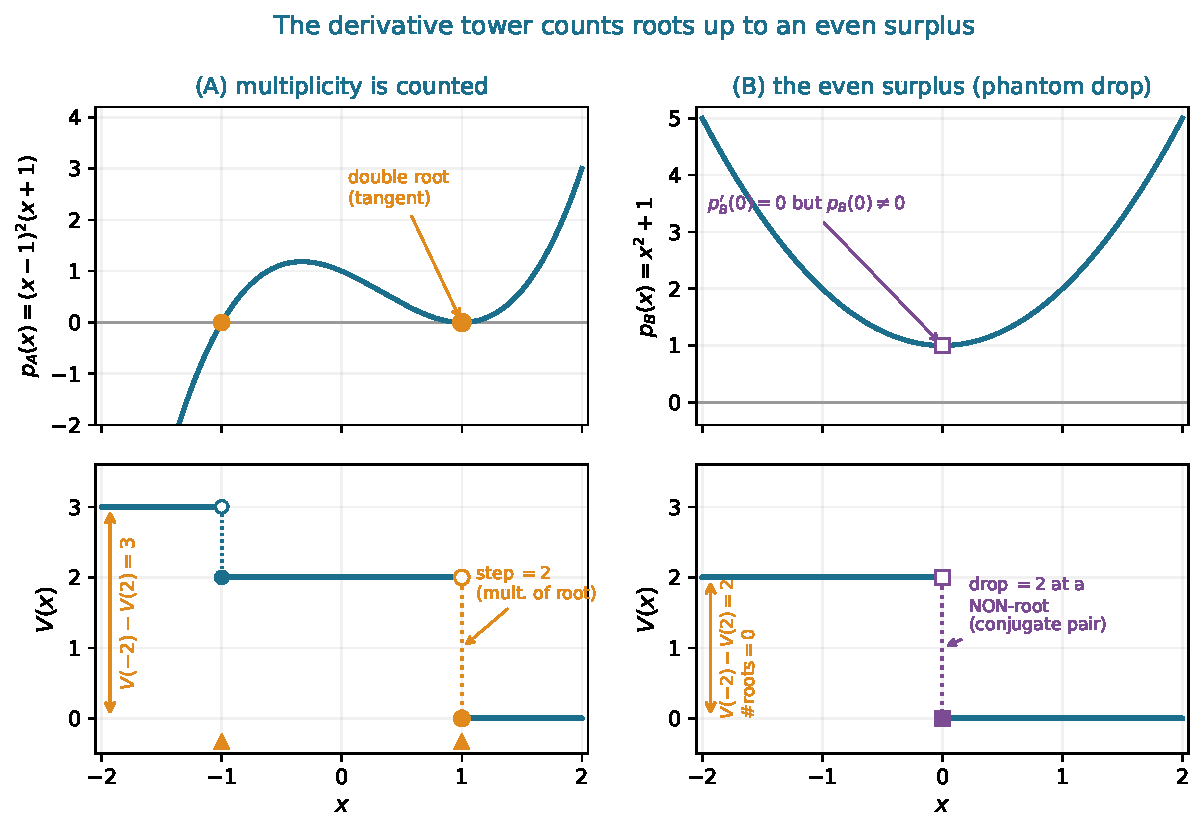
\includegraphics[width=\textwidth]{budan_fig1_tower}
\caption{The derivative tower counts roots up to an even surplus. \emph{(A)} $p_A=(x-1)^2(x+1)$:
$\V$ drops by $1$ at the simple root $x=-1$ and by $2$ at the double root $x=1$ (open circle = the
value just to the left, filled = the value at the point, on the lower step). The descent over
$(-2,2]$ equals the root count \emph{with multiplicity}, so the inequality is sharp. \emph{(B)}
$p_B=x^2+1$, no real root: $\V$ still drops by $2$, at $x=0$, where the interior member $p_B'$
vanishes but $p_B$ does not---the even surplus, the signature of a conjugate pair. Every plotted
sign and count is asserted against exact arithmetic before drawing.}
\label{fig:tower}
\end{figure}

\begin{table}[htbp]
\centering\small
\rowcolors{2}{ggband!35}{white}
\begin{tabular}{@{}rccccr@{}}
\toprule
\rowcolor{ggteal!18}
$x$ & $p_A$ & $p_A'$ & $p_A''$ & $p_A'''$ & $\V(x)$ \\
    & {\scriptsize$x^3{-}x^2{-}x{+}1$} & {\scriptsize$3x^2{-}2x{-}1$} & {\scriptsize$6x{-}2$} & {\scriptsize$6$} & \\
\midrule
$-2$            & $-$ & $+$ & $-$ & $+$ & $3$ \\
$-\tfrac32$     & $-$ & $+$ & $-$ & $+$ & $3$ \\
$-1$ {\scriptsize(root)}        & $0$ & $+$ & $-$ & $+$ & $2$ \\
$0$             & $+$ & $-$ & $-$ & $+$ & $2$ \\
$\tfrac12$      & $+$ & $-$ & $+$ & $+$ & $2$ \\
$1$ {\scriptsize(double root)}  & $0$ & $0$ & $+$ & $+$ & $0$ \\
$2$             & $+$ & $+$ & $+$ & $+$ & $0$ \\
\bottomrule
\end{tabular}
\caption{Example A read off the tower. $\V$ falls by $1$ at the simple root $x=-1$ and by $2$ at the
double root $x=1$: the drop counts multiplicity. On $(-2,2]$, $\V(-2)-\V(2)=3$ equals the root count
with multiplicity, so the Budan--Fourier inequality is sharp here. The whole table is regenerated and
checked in exact arithmetic by \lean{budan\_fig1\_tower.py}.}
\label{tab:signsA}
\end{table}

The picture behind the tables is the staircase that names the paper's method. Plot $\V(x)$ as $x$
sweeps the line: it is flat almost everywhere and drops only at \emph{critical points}---points
where some member of the tower vanishes. At a root of $p$ it drops by the multiplicity; at a
critical point that is not a root of $p$ it can still drop, by an even amount. The whole content of
the next two sections is in proving that the staircase has exactly this shape. That is the bead this
section hands on: \emph{why does $\V$ move only at critical points, and there by precisely the
multiplicity plus an even number?}

\section{Q2: why does the count move only at critical points, and by how much?}\label{sec:q2}

\emph{History bead.} The local analysis is the heart of every proof of Budan--Fourier. What makes it
harder than Sturm's is structural: Sturm's chain is built so that consecutive members are coprime,
so no two of them vanish together and the analysis at a root touches only the leading pair
$(p,p')$. The derivative tower has no such luck---$p$ and $p'$ \emph{do} vanish together at a
multiple root, and a whole \emph{block} of consecutive members $p^{(i)},\dots,p^{(j)}$ can vanish at
one point. The Lean is in the lemmas \lean{sign\_eval\_right\_vanish}, \lean{sign\_eval\_left\_vanish}
(the two bricks) and \lean{fourierVar\_drop\_at\_critical\_point} (their assembly).

Away from critical points every member keeps its sign---a polynomial cannot change sign without a
root, by the intermediate value theorem---so $\V$ is locally constant (\lean{fourierVar\_eq\_of\_no\_root},
inherited verbatim from the Sturm toolkit). That is why the staircase is flat between criticals. All
the action is at a critical point $c$, and the new difficulty is the vanishing block.

\emph{The two bricks.} The tower has one feature that replaces coprimality: each member is the
derivative of the previous one, $p^{(k+1)}=(p^{(k)})'$. So if $p^{(k)}(c)=0$ while $p^{(k+1)}$ keeps a
constant nonzero sign $s$ just off $c$, then $p^{(k)}$ is strictly monotone there, and its sign just
off $c$ is forced---\emph{the same} as its derivative $p^{(k+1)}$ on the right, the \emph{opposite} on
the left. No Taylor expansion, no multiplicity bookkeeping: one application of the mean value theorem.
\begin{recipebox}{The two monotonicity bricks (recipe)}
If $q(c)=0$ and $q'$ keeps the constant nonzero sign $s$ on $(c,z]$, then
$\mathrm{sign}\,q(z)=s$ (\lean{sign\_eval\_right\_vanish}). If instead $q'$ keeps sign $s$ on $[z,c)$,
then $\mathrm{sign}\,q(z)=-s$ (\lean{sign\_eval\_left\_vanish}). Apply this up a vanishing block,
anchored at its first \emph{non}-vanishing member (the higher derivative just past the block):
\textbf{on the right of $c$ each vanishing member copies the sign of its derivative}, so the block
collapses to a single sign and contributes \emph{no} sign change; \textbf{on the left each takes the
opposite of its derivative's sign}, so the block \emph{alternates} and contributes one sign change per
member.
\end{recipebox}

\begin{figure}[htbp]
\centering
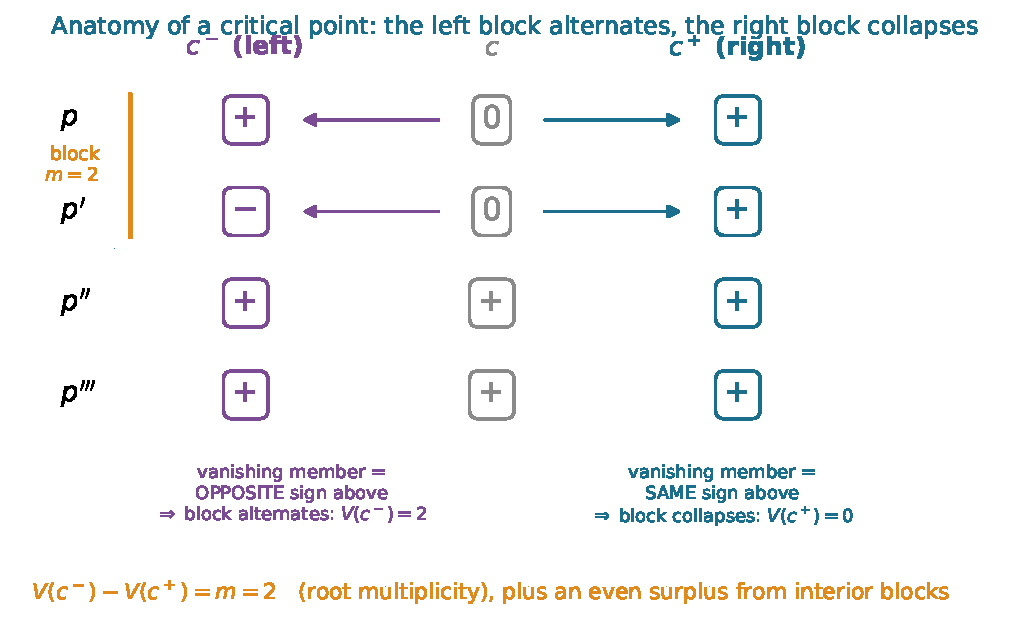
\includegraphics[width=0.74\textwidth]{budan_fig2_critical}
\caption{Anatomy of a critical point, for the double root $c=1$ of $p_A$ (the block $p,p'$ vanishes,
$m=2$). Reading each sign just off $c$ from that member's derivative: on the right (teal)
a vanishing member copies its derivative's sign---the block collapses, $\V(c^+)=0$; on the left (plum)
it takes the opposite---the block alternates, $\V(c^-)=2$. Hence $\V(c^-)-\V(c^+)=m$, the multiplicity, plus
an even amount from any interior blocks. Signs are exact from the tower of $p_A$.}
\label{fig:critical}
\end{figure}

Counting the consequences gives the local drop. Just right of $c$ the tower's sign list is the list
at $c$ with each vanishing entry replaced by the sign of its first nonvanishing successor---an
operation on bare sign lists I call \lean{Rseq}; just left of $c$ it is the same with
\emph{alternating} signs, \lean{Lseq}. The right list has the \emph{same} number of sign changes as
the list at $c$ (\lean{Rseq\_spec}: $\V(c^+)=\V(c)$, the right side carries no information); the left
list has that many \emph{plus} the length of the leading vanishing run \emph{plus} an even surplus
from interior blocks (\lean{Lseq\_spec}). Writing $m$ for the leading run and packaging the surplus
as $2e$,
\keyeq{\V(c^-)\ =\ \V(c^+)\ +\ m\ +\ 2e .}
Figure~\ref{fig:critical} shows the mechanism on the double root of $p_A$, where the block $p,p'$
gives $\V(1^-)-\V(1^+)=2$. The last step is to recognize $m$: the leading run of vanishing members at
$c$ has length exactly the \emph{root multiplicity} of $p$ at $c$, because in characteristic zero the
order of the first nonvanishing derivative \emph{is} the multiplicity. Mathlib knows this
(\lean{lt\_rootMultiplicity\_iff\_isRoot\_iterate\_derivative}), and the roots of $p$ in $(a,b]$ that
sit at $c$ number exactly that multiplicity (\lean{count\_roots}). So $m=\#\mathrm{roots}(a,b]$ at a
genuine root, and $m=0$ at a critical point that is not a root---in which case the whole drop is the
even surplus, exactly Example B. The additive form $\V(a)=\V(b)+\#\mathrm{roots}+2e$ packages the
inequality and the parity into one statement that will add cleanly across the interval.

The bead this hands on is the one the machine cares about most: \emph{this whole picture is a
sentence on paper---``the left block alternates and the right collapses''---but where, made formal,
does it resist?}

\section{Q3: where does the proof resist being made formal?}\label{sec:q3}

\emph{History bead.} On paper the block analysis is a picture; made formal, it is the one genuinely
structural step, because the alternation and the collapse must be performed \emph{along a list whose
shape is recursive}, and the hypotheses that justify each step---which member vanishes, what sign its
neighbour has---are threaded through the tower's own structure. The device that resolves it, the pair
\lean{Rseq}/\lean{Lseq} together with their specifications, is the part of this development with the
least direct textbook antecedent: not a new theorem, but the proof engineering that keeps the
bookkeeping honest. It is the tower's analogue of the \lean{FlankReduce} relation that did the same
job for Sturm~\cite{sturmlean}.

The difficulty is precise. To compare $\V(a)$ with $\V(b)$ across $c$, one must perform the
collapse-on-the-right and alternate-on-the-left on the evaluated sign lists, and the rule for each
entry depends on whether \emph{that} member vanishes at $c$ and on the sign of its derivative.
The combinatorics of rewriting a list and the algebra of why each rewrite is legal are entangled, and
an honest proof separates them.

The separation is two list operations on bare signs, defined by recursion and proved correct without
ever mentioning a polynomial.
\begin{recipebox}{The decoupling (recipe)}
On a list $s$ of signs (entry $0$ = a vanishing member, $\pm1$ = a kept one), \lean{Rseq} replaces
each $0$ by the next surviving value and \lean{Lseq} replaces it by the negation of that value.
Two facts then divide the labour. \emph{Combinatorial:} \lean{Rseq\_spec} shows the right list has the
same sign-change count as $s$, and \lean{Lseq\_spec} shows the left list has that count plus the
leading-zero run plus an even number---this is pure list induction carrying a head sign-parity
invariant, no polynomials. \emph{Structural:} \lean{signs\_right\_eq\_Rseq} and
\lean{signs\_left\_eq\_Lseq} show that the tower's evaluated sign list at $b$ (resp.\ $a$) \emph{is}
\lean{Rseq} (resp.\ \lean{Lseq}) of the list at $c$---this is the induction over the tower, fed by the
two monotonicity bricks and by nothing else.
\end{recipebox}

\begin{figure}[htbp]
\centering
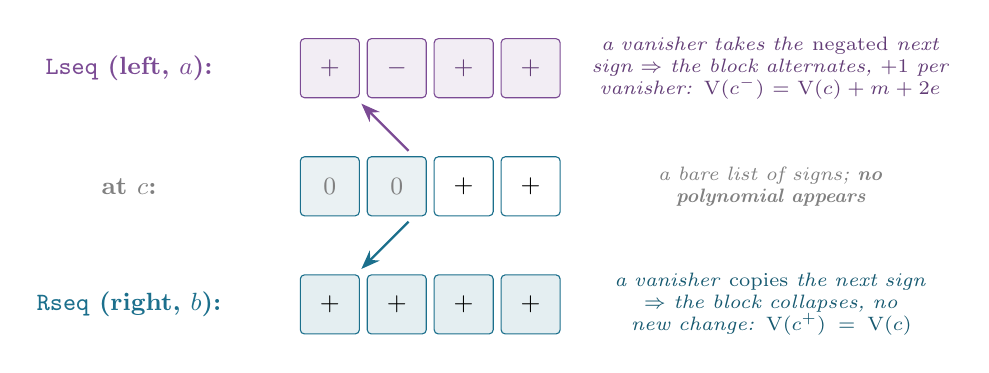
\begin{tikzpicture}[
  s/.style={draw=ggteal,rounded corners=1.5pt,minimum size=7.5mm,inner sep=2pt,font=\small,fill=white},
  sz/.style={draw=ggteal,rounded corners=1.5pt,minimum size=7.5mm,inner sep=2pt,font=\small,
    fill=ggband!60,text=gray},
  sl/.style={draw=ggplum,rounded corners=1.5pt,minimum size=7.5mm,inner sep=2pt,font=\small,
    fill=ggplum!10,text=ggplum!80!black},
  sr/.style={draw=ggteal,rounded corners=1.5pt,minimum size=7.5mm,inner sep=2pt,font=\small,
    fill=ggteal!12},
  arr/.style={-{Stealth[length=2.4mm]},thick},
  lbl/.style={font=\scriptsize\itshape,align=center}]
  % centre: the list AT c
  \node[font=\bfseries\small,text=gray] at (-2.55,0) {at $c$:};
  \node[sz] (c0) at (0,0) {$0$};
  \node[sz] (c1) at (0.85,0) {$0$};
  \node[s]  (c2) at (1.70,0) {$+$};
  \node[s]  (c3) at (2.55,0) {$+$};
  % left: Lseq (negate the entry below) -> alternates
  \node[font=\bfseries\small,text=ggplum] at (-2.55,1.5) {$\lean{Lseq}$ (left, $a$):};
  \node[sl] at (0,1.5) {$+$};
  \node[sl] at (0.85,1.5) {$-$};
  \node[sl] at (1.70,1.5) {$+$};
  \node[sl] at (2.55,1.5) {$+$};
  % right: Rseq (copy the entry below) -> collapses
  \node[font=\bfseries\small,text=ggteal] at (-2.55,-1.5) {$\lean{Rseq}$ (right, $b$):};
  \node[sr] at (0,-1.5) {$+$};
  \node[sr] at (0.85,-1.5) {$+$};
  \node[sr] at (1.70,-1.5) {$+$};
  \node[sr] at (2.55,-1.5) {$+$};
  \draw[arr,ggplum] (1.0,0.45) -- (0.4,1.05);
  \draw[arr,ggteal] (1.0,-0.45) -- (0.4,-1.05);
  \node[lbl,text=ggplum!80!black,text width=4.6cm] at (5.6,1.5)
    {a vanisher takes the \emph{negated} next sign $\Rightarrow$ the block alternates,
     $+1$ per vanisher: $\V(c^-)=\V(c)+m+2e$};
  \node[lbl,text=ggteal!80!black,text width=4.6cm] at (5.6,-1.5)
    {a vanisher \emph{copies} the next sign $\Rightarrow$ the block collapses, no new change:
     $\V(c^+)=\V(c)$};
  \node[lbl,text=gray,text width=4.6cm] at (5.6,0)
    {a bare list of signs; \textbf{no polynomial appears}};
\end{tikzpicture}
\caption{The decoupling of Section~\ref{sec:q3}, at the level of bare sign lists (here the block
$0,0$ of the double root of $p_A$). \lean{Rseq} and \lean{Lseq} are pure list operations---a
vanishing entry copies, resp.\ negates, the next surviving sign---and their counting
specifications (\lean{Rseq\_spec}, \lean{Lseq\_spec}) are proved by list induction with no polynomial
in sight. The structural lemmas \lean{signs\_right\_eq\_Rseq}/\lean{signs\_left\_eq\_Lseq} are the only
bridge back to the tower, and they are fed solely by the two monotonicity bricks.}
\label{fig:decouple}
\end{figure}

Three smaller frictions are worth naming, because each is a place the machine refused a hand-wave.
\emph{First}, the tower's recursive structure had to be made explicit: that consecutive members are
related by differentiation is the hypothesis \lean{List.IsChain}, and the bricks consume it one step
at a time as the induction walks down a block. \emph{Second}, the multiplicity step is not a
definition but a theorem, and a nontrivial one---that the leading vanishing run equals the root
multiplicity rests on Mathlib's characterization of multiplicity by iterated derivatives, and on
identifying the first \emph{non}-vanishing member as the top of the tower, a nonzero constant, so the
run always terminates. \emph{Third}, a small but real Lean trap: rewriting under \lean{List.getLast},
whose value carries a proof that the list is nonempty, is not a plain \lean{rw}; the dependency forces
\lean{simp} or an explicit congruence.

\emph{What the machine made me state correctly.} As with Sturm, formalizing forbade the genericity
hand-wave---``slide the endpoints to non-critical points''---and rewarded stating the local drop at
the weakest honest level. \lean{fourierVar\_drop\_at\_critical\_point} is proved for a critical point
$c$ anywhere in the \emph{closed} interval $[a,b]$, endpoints included. The endpoint cases are not
special pleading: when $c=a$ the interval $(a,b]$ excludes it and the local count is the even surplus
with no multiplicity term; when $c=b$ the same additive identity holds with the multiplicity carried
by the leading run. Both fall out of the one statement, discharged by the same lines as the interior
case---the principle the companion paper on Newton's inequalities~\cite{newton} also drew: the
weakest honest generality dissolves edge cases rather than multiplying them.

\emph{From one step to the whole staircase.} The global theorem is then an induction on the number of
\emph{distinct} critical points in $(a,b]$ (the roots of the product of all tower members, a nonzero
polynomial, hence finite). Peel off the largest critical point $c$; choose a non-critical separator
$d$ just below it; apply the per-point drop on $[d,b]$, where $c$ is the only critical point; recurse
on $[a,d]$. The half-open interval splits as $(a,d]\sqcup(d,b]$, the multiplicity-aware root count
adds (\lean{rootCount\_split}), and the two additive existentials combine into one. The bead handed on:
\emph{now that the theorem is certified, what does the library get for free?}

\section{Q4: what becomes free once the theorem is certified?}\label{sec:q4}

\emph{History bead.} Budan's rule and Fourier's theorem are, between them, the bridge from Descartes'
coefficient count to interval methods; the modern algorithmic descendants are the continued-fraction
and bisection real-root isolators of Vincent, Collins and Akritas~\cite{vincent,collinsakritas}. The
parity refinement is the part that explains the others.

\emph{Descartes, and why it overcounts evenly.} Descartes' rule is the shadow of Budan--Fourier on
$(0,\infty)$. At the left end the tower evaluates to $p^{(k)}(0)=k!\,a_k$, where $a_k$ is the
coefficient of $x^k$; so the tower's sign sequence at $0$ \emph{is} the sign sequence of the
coefficients, and $\V(0)$ is exactly the coefficient sign-variation count Mathlib already computes. At
the other end every $p^{(k)}$ takes the sign of the one leading coefficient, so $\V(+\infty)=0$.
Budan--Fourier on $(0,\infty)$ then reads: the number of positive roots is at most
$\V(0)-\V(+\infty)=\V(0)$, the coefficient sign variations, and differs from it by an even number. That
even number is the content---it is why Descartes' rule never reports a parity error:
\textbf{the unseen roots come in conjugate pairs, and each pair contributes $2$ to the gap}.
Figure~\ref{fig:shadow} is the smallest instance carrying a pair: for $p=(x^2+1)(x-1)$ the
coefficients $+,-,+,-$ give $\V(0)=3$, there is a single positive root $x=1$, and the gap $2$ is
exactly the conjugate pair $\pm i$. The Lean count used here and Mathlib's
\lean{Polynomial.signVariations} are, after unfolding, the same kind of object, so the toolkit
transfers; what the tower adds over the coefficients is precisely the interval and the localization of
the even gap.

\begin{figure}[htbp]
\centering
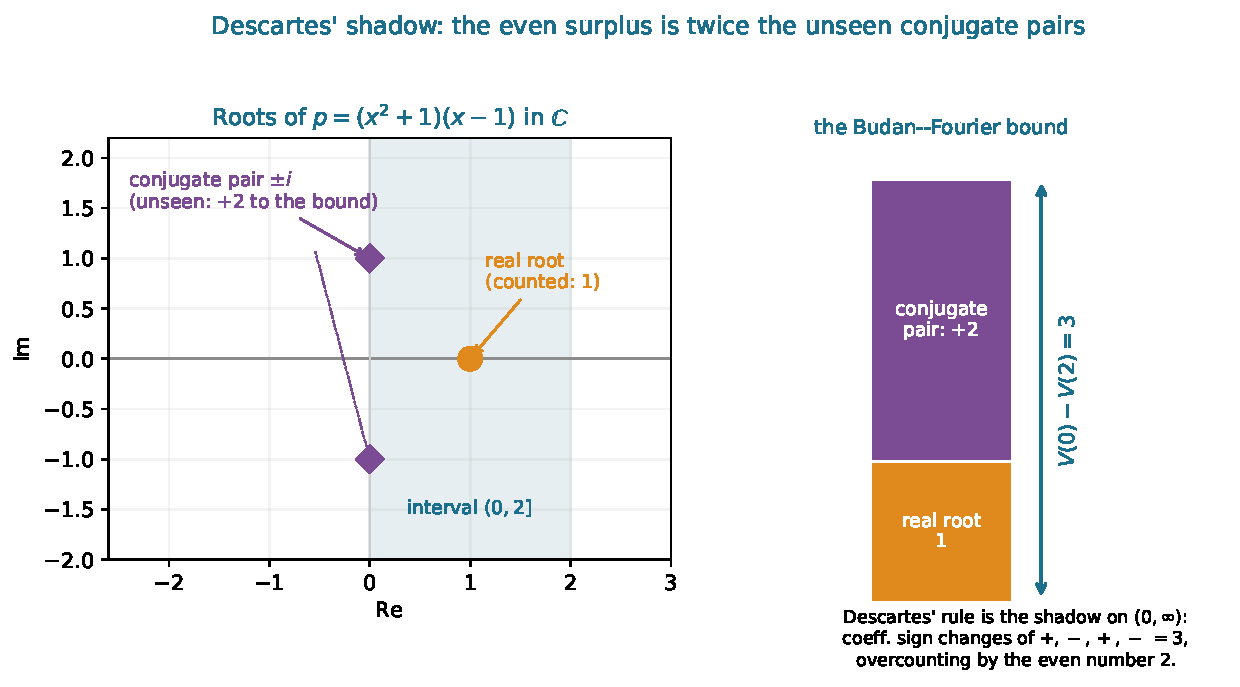
\includegraphics[width=0.88\textwidth]{budan_fig3_shadow}
\caption{Descartes' shadow. For $p=(x^2+1)(x-1)$ on $(0,2]$ the tower drop is $\V(0)-\V(2)=3$: the
single real root $x=1$ contributes $1$, and the unseen conjugate pair $\pm i$ contributes the even
remainder $2$. Read on $(0,\infty)$ this is Descartes' rule---three coefficient sign changes
$+,-,+,-$, overcounting the one positive root by an even number. The surplus is always even because
the complex roots of a real polynomial come in conjugate pairs. Counts asserted exactly before
drawing.}
\label{fig:shadow}
\end{figure}

\emph{The companion of Sturm.} The two theorems now sit side by side in the same Lean development,
built on one sign-variation toolkit: Sturm's exact count of \emph{distinct} roots on the remainder
chain~\cite{sturmlean}, and Budan--Fourier's multiplicity-aware bound on the derivative tower. The
shared core---local constancy, the recursive sign-change count, the leading-pair recursion---was
written once and used twice. Their difference is now a formal object too: Sturm's chain is coprime and
its local analysis is a single head-drop; the tower is not, and its local analysis is the block
collapse of Section~\ref{sec:q2}.

\section{What a certified Budan--Fourier enables}\label{sec:enables}

Beyond Descartes, the certified theorem is the first verified step of the classical bridge to
real-root isolation. A subdivision method that bisects an interval and reads $\V(a)-\V(b)$ on each
half has, in this theorem, a machine-checked guarantee that the reported number is an upper bound on
the roots and that it drops to the true count as the intervals shrink around simple roots; the
multiplicity-aware version is exactly what isolation of multiple roots needs. Wenda Li's Isabelle
development~\cite{liBF} took this route to a verified root-counting procedure; the Lean pieces here
are the foundation on which the same could be built over Mathlib. Nothing in this paper builds the
isolator---that is named honestly among the open questions---but the load-bearing lemma it would
stand on is now in the library.

\section{The building blocks}\label{sec:blocks}

Table~\ref{tab:results} gathers the load-bearing results, all \lean{sorry}-free in
\lean{BudanFourier.lean}; Table~\ref{tab:signsB} reads Example B off its tower, the smallest witness of
the even surplus; Table~\ref{tab:metrics} measures the development. The dependency runs as the
reader's map (Figure~\ref{fig:readermap}): the two monotonicity bricks feed the per-member sign
recursions, which feed \lean{signs\_right\_eq\_Rseq}/\lean{signs\_left\_eq\_Lseq}; these, with the
pure-list \lean{Rseq\_spec}/\lean{Lseq\_spec} and the multiplicity identification, give the local
drop \lean{fourierVar\_drop\_at\_critical\_point}; and the global induction over critical points
assembles \lean{budan\_fourier}.

\begin{table}[H]
  \centering\small
  \arrayrulecolor{ggteal}
  \begin{tabular}{@{}llc@{}}
    \toprule
    \rowcolor{ggteal}
    \textcolor{white}{\textbf{Lean name}} & \textcolor{white}{\textbf{Statement}} & \textcolor{white}{\textbf{Status}} \\
    \midrule
    \rowcolor{ggband}
    \lean{budan\_fourier} & $\#\mathrm{roots}(a,b]\le \V(a){-}\V(b)$ and $\V(a){-}\V(b){-}\#\mathrm{roots}$ even & proven \\
    \lean{fourierVar\_drop\_at\_critical\_point} & $\exists e,\ \V(a)=\V(b)+\#\mathrm{roots}(a,b]+2e$ (local core) & proven \\
    \rowcolor{ggband}
    \lean{fourierVar\_eq\_signVarAt} & $\V_p(x)=\lean{signVarAt}\,(\lean{fourierSeq}\,p)\,x$ (bridge, \lean{rfl}) & proven \\
    \lean{signs\_right\_eq\_Rseq} & signs at $b$ $=\lean{Rseq}$ of signs at $c$ (right collapses) & proven \\
    \rowcolor{ggband}
    \lean{signs\_left\_eq\_Lseq} & signs at $a$ $=\lean{Lseq}$ of signs at $c$ (left alternates) & proven \\
    \lean{Rseq\_spec} / \lean{Lseq\_spec} & $\V(c^+){=}\V(c)$;\ $\V(c^-){=}\V(c^+){+}m{+}2g$ (combinatorial) & proven \\
    \rowcolor{ggband}
    \lean{fourierSeq\_isChain} & the tower is a derivative chain $p^{(k+1)}=(p^{(k)})'$ & proven \\
    \lean{sign\_eval\_\{right,left\}\_vanish} & the two monotonicity bricks (sign just off a root) & proven \\
    \bottomrule
  \end{tabular}
  \arrayrulecolor{black}
  \caption{The load-bearing results, all \lean{sorry}-free in \lean{BudanFourier.lean} (Lean~4 /
  Mathlib). \lean{\#print axioms BudanFourier.budan\_fourier} reports only \lean{propext},
  \lean{Classical.choice}, \lean{Quot.sound}. To the best of my knowledge this is the first
  formalization of the Budan--Fourier theorem in Lean.}
  \label{tab:results}
\end{table}

\begin{table}[H]
\centering\small
\rowcolors{2}{ggband!35}{white}
\begin{tabular}{@{}rcccr@{}}
\toprule
\rowcolor{ggteal!18}
$x$ & $p_B=x^2{+}1$ & $p_B'=2x$ & $p_B''=2$ & $\V(x)$ \\
\midrule
$-2$            & $+$ & $-$ & $+$ & $2$ \\
$-1$            & $+$ & $-$ & $+$ & $2$ \\
$0$ {\scriptsize($p_B'{=}0$, not a root)} & $+$ & $0$ & $+$ & $0$ \\
$1$             & $+$ & $+$ & $+$ & $0$ \\
$2$             & $+$ & $+$ & $+$ & $0$ \\
\bottomrule
\end{tabular}
\caption{Example B, $p_B=x^2+1$, with no real root. $\V$ drops by $2$ at $x=0$---a zero of the
interior member $p_B'$, \emph{not} a root of $p_B$. Thus $\#\mathrm{roots}(-2,2]=0<\V(-2)-\V(2)=2$
and the surplus is even: the signature of a conjugate pair, and exactly the
\lean{fourierVar\_drop\_at\_critical\_point} case with witness $e=1$.}
\label{tab:signsB}
\end{table}

\begin{table}[H]
  \centering\small
  \arrayrulecolor{ggteal}
  \begin{tabular}{@{}lr@{}}
    \toprule
    \rowcolor{ggteal}
    \textcolor{white}{\textbf{Quantity}} & \textcolor{white}{\textbf{Value}} \\
    \midrule
    \rowcolor{ggband}
    Lines in \lean{BudanFourier.lean} & $940$ \\
    Theorems / definitions & $28$ \\
    \rowcolor{ggband}
    \lean{sorry} / \lean{admit} / \lean{native\_decide} & $0$ \\
    Axioms beyond Lean's core & $0$ \\
    \rowcolor{ggband}
    Reused from \lean{Sturm.lean} & sign-variation toolkit \\
    Compile time (warm Mathlib) & ${\approx}\,8$\,s \\
    \bottomrule
  \end{tabular}
  \arrayrulecolor{black}
  \caption{The development measured. Compile time is for checking \lean{BudanFourier.lean} against a
  prebuilt Mathlib and the imported \lean{Sturm} library, whose sign-variation toolkit is reused.}
  \label{tab:metrics}
\end{table}

\section{The boundary of the contribution}\label{sec:boundary}

I want the limits stated without varnish.

\emph{Not first in any system.} The Budan--Fourier theorem was formalized in Isabelle/HOL by Wenda
Li in 2018--2019~\cite{liBF}, with multiplicity, and used there to drive a verified root-counting
procedure; Li also extended a prior Isabelle formalization of Sturm's theorem to count with
multiplicity. The present work is, to the best of my knowledge, the first proof in \emph{Lean}, based
on searches of Loogle and a \lean{grep} of Mathlib in June~2026. The value is the Lean-and-Mathlib
formalization and its reusable machinery, not priority over Isabelle.

\emph{The field and characteristic.} Everything is over $\R$. The multiplicity step uses
characteristic zero in an essential way---it is what makes the order of the first nonvanishing
derivative equal the root multiplicity---so the proof as written does not transfer verbatim to
positive characteristic, where that identity fails.

\emph{What is and is not counted.} The theorem counts roots with multiplicity and bounds them by the
sign-variation drop, with the even-parity refinement. It does \emph{not} compute the roots, does not
produce a certificate of the count for a downstream tool, and does not build a root isolator; those are
named among the open questions.

\emph{What is reused versus new.} The sign-variation toolkit---local constancy, \lean{signChanges},
the leading-pair recursion---is imported from the Sturm development~\cite{sturmlean} and not
re-derived. New here are the two monotonicity bricks, the \lean{Rseq}/\lean{Lseq} decoupling and their
specifications, the identification of the leading run with the multiplicity, and the assembly into the
local drop and the global theorem.

\section{Reflective questions, for the next bead}\label{sec:questions}

A string of beads is meant to be continued. Machine-checking a two-hundred-year-old theorem is not an
end in itself: its worth is measured by what the certified pieces let one ask next, and ask more
sharply. I close with the questions I would rather carry forward than pretend to have settled---each a
place where this work stops short, and each, I think, not just the seed of another paper but a rung up
from this one.

\begin{enumerate}\itemsep3pt
\item \emph{From bound to certificate.} The theorem says the drop \emph{bounds} the count and shares
its parity; the even surplus measures how far the bound overshoots. Can the surplus be made into a
\emph{computation}---a verified procedure that, by bisecting until the surplus vanishes, returns the
exact multiplicity-aware root count, and a certificate a skeptical tool can re-check? How much of the
continued-fraction machinery of Vincent and Akritas~\cite{vincent,collinsakritas} would the honest
bridge want?

\item \emph{Porting the known unification, not claiming it.} That Descartes', Budan--Fourier's and
Sturm's counts are facets of one sign-variation principle is classical, not mine---it is said plainly by
Akritas~\cite{akritas} and Basu--Pollack--Roy~\cite{bpr}---and the deeper unifying invariant, the
\emph{Cauchy index}, is axiomatised through abstract \emph{Sturm chains} by Eisermann~\cite{eisermann}
and has \emph{already} been machine-checked, in Isabelle/HOL, by Li and Paulson~\cite{liCauchy}. What is
missing is a \emph{Lean} formalisation of that framework. One sub-question, though, is genuinely open and
specific to this work: the derivative tower's \emph{vanishing blocks} break the coprimality the classical
Sturm-chain axioms lean on---do they still satisfy those axioms, or do they force a strictly weaker
axiom set in which the collapse/alternation of Section~\ref{sec:q2} is the general local law (so that
\lean{Rseq}/\lean{Lseq} are the primitive and \lean{FlankReduce} a degenerate case)? The honest target
is to carry a known unification into Mathlib, and to find the weakest axioms the tower forces.

\item \emph{What the decoupling really is.} \lean{Rseq}/\lean{Lseq} separated the combinatorics of
rewriting a sign list from the algebra licensing each rewrite, exactly as \lean{FlankReduce} did for
Sturm. Two different chains, the same shape of argument: is ``a sign-change tally transformed by a
locally-licensed list rewrite'' a reusable lemma in its own right, or did it merely fit twice? I
suspect the former and have not proved it.

\item \emph{The block, beyond characteristic zero and beyond one variable.} The multiplicity step
leans on characteristic zero; the tower itself does not. What is the right statement over a general
field, where the leading run need not equal the multiplicity? And is there a Bernstein-basis or
multivariate analogue of the block collapse---the place where root counting on the line meets the
geometry of several variables?
\end{enumerate}

\noindent What ties the four together is one reflection. With the theorem now a fixed point that a
kernel will defend, the interesting direction is no longer proving it again but asking what can stand
\emph{on} it: a certificate, a single principle behind three counts, a reusable proof pattern, a wider
field. Each would not merely extend the result---it would raise the whole derivative-tower story by a
level, which is the only kind of continuation worth the next bead.

\section*{Reproducing}
\begin{verbatim}
git clone https://github.com/karlesmarin/godsil-gutman-lean
cd godsil-gutman-lean && lake exe cache get
lake build Sturm           # the imported sign-variation toolkit
lake env lean BudanFourier.lean
\end{verbatim}
Lean \lean{v4.30.0-rc2}, Mathlib pin \lean{701fb6e9}. The theorem is \lean{BudanFourier.budan\_fourier}
in \lean{BudanFourier.lean}; its supports are in Table~\ref{tab:results}. It is checked by \lean{\#print
axioms} to depend only on \lean{propext}, \lean{Classical.choice}, \lean{Quot.sound}. The worked
examples of Figures~\ref{fig:tower} and~\ref{fig:critical} are re-derived, and every sign and count
asserted against exact arithmetic, before the figures are drawn (\lean{figures/budan\_fig1\_tower.py},
\lean{figures/budan\_fig2\_critical.py}).

\begin{thebibliography}{99}\small
\bibitem{descartes} R.~Descartes, \emph{La G\'eom\'etrie} (1637); the rule of signs bounds the number
of positive roots by the number of sign changes of the coefficients.
\bibitem{budan} F.~D.~Budan de Boislaurent, \emph{Nouvelle m\'ethode pour la r\'esolution des
\'equations num\'eriques}, Paris (1807; 2nd ed.\ 1822).
\bibitem{fourier} J.~Fourier, \emph{Analyse des \'equations d\'etermin\'ees}, Firmin Didot, Paris
(posthumous, 1831).
\bibitem{sturm} C.~Sturm, M\'emoire sur la r\'esolution des \'equations num\'eriques, \emph{M\'emoires
pr\'esent\'es par divers savants \`a l'Acad\'emie Royale des Sciences} \textbf{6} (1835) 271--318;
presented in 1829.
\bibitem{akritas} A.~G.~Akritas, Reflections on a pair of theorems by Budan and Fourier, \emph{Mathematics
Magazine} \textbf{55} (1982) 292--298.
\bibitem{collinsakritas} G.~E.~Collins, A.~G.~Akritas, Polynomial real root isolation using Descartes'
rule of signs, in \emph{Proc.\ SYMSAC~'76}, ACM, 1976, 272--275.
\bibitem{vincent} A.~Alesina, M.~Galuzzi, A new proof of Vincent's theorem, \emph{L'Enseignement
Math\'ematique} \textbf{44} (1998) 219--256.
\bibitem{bpr} S.~Basu, R.~Pollack, M.-F.~Roy, \emph{Algorithms in Real Algebraic Geometry}, 2nd ed.,
Algorithms and Computation in Mathematics \textbf{10}, Springer, 2006 (sign-variation theory, Ch.~2).
\bibitem{eisermann} M.~Eisermann, The fundamental theorem of algebra made effective: an elementary
real-algebraic proof via Sturm chains, \emph{Amer.\ Math.\ Monthly} \textbf{119} (2012), no.~9,
715--752; \texttt{arXiv:0808.0097} (abstract ``Sturm chains'' and the Cauchy index).
\bibitem{liBF} W.~Li, L.~C.~Paulson, Counting polynomial roots in Isabelle/HOL: a formal proof of the
Budan--Fourier theorem, in \emph{Proc.\ 8th ACM SIGPLAN Int.\ Conf.\ on Certified Programs and Proofs
(CPP~2019)}, ACM, 2019, 52--64 (\texttt{doi:10.1145/3293880.3294092}); preprint
\texttt{arXiv:1811.11093}. The accompanying Archive of Formal Proofs entry ``The Budan--Fourier Theorem
and Counting Real Roots with Multiplicity'' (W.~Li, 2018), \url{https://isa-afp.org/entries/Budan_Fourier.html}.
\bibitem{litarski} W.~Li, L.~C.~Paulson, A formal proof of the Sturm--Tarski theorem, \emph{Archive of
Formal Proofs} (2014), \url{https://isa-afp.org/entries/Sturm_Tarski.html}.
\bibitem{liCauchy} W.~Li, L.~C.~Paulson, Evaluating winding numbers and counting complex roots through
Cauchy indices in Isabelle/HOL, \emph{J.~Automated Reasoning} \textbf{64} (2020), no.~2, 331--360;
\texttt{arXiv:1804.03922}.
\bibitem{eberl} M.~Eberl, Sturm's Theorem, \emph{Archive of Formal Proofs} (2014),
\url{https://isa-afp.org/entries/Sturm_Sequences.html}.
\bibitem{cohen} C.~Cohen, Construction of real algebraic numbers in Coq, in \emph{Interactive Theorem
Proving (ITP 2012)}, LNCS \textbf{7406}, Springer, 2012, 67--82.
\bibitem{mathlib} The mathlib Community, The Lean mathematical library, in \emph{Certified Programs and
Proofs (CPP 2020)}, ACM, 2020, 367--381.
\bibitem{lean4} L.~de Moura, S.~Ullrich, The Lean~4 theorem prover and programming language, in
\emph{Automated Deduction (CADE~28)}, LNCS \textbf{12699}, Springer, 2021, 625--635.
\bibitem{sturmlean} C.~Mar\'in, \emph{The Staircase of Signs: Sturm's Root-Counting Theorem,
Machine-Checked in Lean~4}, Zenodo, 2026, \texttt{doi:10.5281/zenodo.20707348}.
\bibitem{newton} C.~Mar\'in, \emph{The Inward Bow of a Real-Rooted Polynomial: Newton's Inequalities,
Machine-Checked in Lean~4}, Zenodo, 2026, \texttt{doi:10.5281/zenodo.20693064}.
\bibitem{gglean} C.~Mar\'in, \emph{Random Signs into Matchings: A Godsil--Gutman Identity, Formalized
in Lean~4}, Zenodo, 2026, \texttt{doi:10.5281/zenodo.20517350}.
\end{thebibliography}

\end{document}
